% Options for packages loaded elsewhere
% Options for packages loaded elsewhere
\PassOptionsToPackage{unicode}{hyperref}
\PassOptionsToPackage{hyphens}{url}
\PassOptionsToPackage{dvipsnames,svgnames,x11names}{xcolor}
%
\documentclass[
  letterpaper,
  DIV=11,
  numbers=noendperiod]{scrartcl}
\usepackage{xcolor}
\usepackage[top=20mm,bottom=20mm,left=20mm,right=20mm,heightrounded]{geometry}
\usepackage{amsmath,amssymb}
\setcounter{secnumdepth}{5}
\usepackage{iftex}
\ifPDFTeX
  \usepackage[T1]{fontenc}
  \usepackage[utf8]{inputenc}
  \usepackage{textcomp} % provide euro and other symbols
\else % if luatex or xetex
  \usepackage{unicode-math} % this also loads fontspec
  \defaultfontfeatures{Scale=MatchLowercase}
  \defaultfontfeatures[\rmfamily]{Ligatures=TeX,Scale=1}
\fi
\usepackage{lmodern}
\ifPDFTeX\else
  % xetex/luatex font selection
\fi
% Use upquote if available, for straight quotes in verbatim environments
\IfFileExists{upquote.sty}{\usepackage{upquote}}{}
\IfFileExists{microtype.sty}{% use microtype if available
  \usepackage[]{microtype}
  \UseMicrotypeSet[protrusion]{basicmath} % disable protrusion for tt fonts
}{}
\makeatletter
\@ifundefined{KOMAClassName}{% if non-KOMA class
  \IfFileExists{parskip.sty}{%
    \usepackage{parskip}
  }{% else
    \setlength{\parindent}{0pt}
    \setlength{\parskip}{6pt plus 2pt minus 1pt}}
}{% if KOMA class
  \KOMAoptions{parskip=half}}
\makeatother
% Make \paragraph and \subparagraph free-standing
\makeatletter
\ifx\paragraph\undefined\else
  \let\oldparagraph\paragraph
  \renewcommand{\paragraph}{
    \@ifstar
      \xxxParagraphStar
      \xxxParagraphNoStar
  }
  \newcommand{\xxxParagraphStar}[1]{\oldparagraph*{#1}\mbox{}}
  \newcommand{\xxxParagraphNoStar}[1]{\oldparagraph{#1}\mbox{}}
\fi
\ifx\subparagraph\undefined\else
  \let\oldsubparagraph\subparagraph
  \renewcommand{\subparagraph}{
    \@ifstar
      \xxxSubParagraphStar
      \xxxSubParagraphNoStar
  }
  \newcommand{\xxxSubParagraphStar}[1]{\oldsubparagraph*{#1}\mbox{}}
  \newcommand{\xxxSubParagraphNoStar}[1]{\oldsubparagraph{#1}\mbox{}}
\fi
\makeatother

\usepackage{color}
\usepackage{fancyvrb}
\newcommand{\VerbBar}{|}
\newcommand{\VERB}{\Verb[commandchars=\\\{\}]}
\DefineVerbatimEnvironment{Highlighting}{Verbatim}{commandchars=\\\{\}}
% Add ',fontsize=\small' for more characters per line
\usepackage{framed}
\definecolor{shadecolor}{RGB}{241,243,245}
\newenvironment{Shaded}{\begin{snugshade}}{\end{snugshade}}
\newcommand{\AlertTok}[1]{\textcolor[rgb]{0.68,0.00,0.00}{#1}}
\newcommand{\AnnotationTok}[1]{\textcolor[rgb]{0.37,0.37,0.37}{#1}}
\newcommand{\AttributeTok}[1]{\textcolor[rgb]{0.40,0.45,0.13}{#1}}
\newcommand{\BaseNTok}[1]{\textcolor[rgb]{0.68,0.00,0.00}{#1}}
\newcommand{\BuiltInTok}[1]{\textcolor[rgb]{0.00,0.23,0.31}{#1}}
\newcommand{\CharTok}[1]{\textcolor[rgb]{0.13,0.47,0.30}{#1}}
\newcommand{\CommentTok}[1]{\textcolor[rgb]{0.37,0.37,0.37}{#1}}
\newcommand{\CommentVarTok}[1]{\textcolor[rgb]{0.37,0.37,0.37}{\textit{#1}}}
\newcommand{\ConstantTok}[1]{\textcolor[rgb]{0.56,0.35,0.01}{#1}}
\newcommand{\ControlFlowTok}[1]{\textcolor[rgb]{0.00,0.23,0.31}{\textbf{#1}}}
\newcommand{\DataTypeTok}[1]{\textcolor[rgb]{0.68,0.00,0.00}{#1}}
\newcommand{\DecValTok}[1]{\textcolor[rgb]{0.68,0.00,0.00}{#1}}
\newcommand{\DocumentationTok}[1]{\textcolor[rgb]{0.37,0.37,0.37}{\textit{#1}}}
\newcommand{\ErrorTok}[1]{\textcolor[rgb]{0.68,0.00,0.00}{#1}}
\newcommand{\ExtensionTok}[1]{\textcolor[rgb]{0.00,0.23,0.31}{#1}}
\newcommand{\FloatTok}[1]{\textcolor[rgb]{0.68,0.00,0.00}{#1}}
\newcommand{\FunctionTok}[1]{\textcolor[rgb]{0.28,0.35,0.67}{#1}}
\newcommand{\ImportTok}[1]{\textcolor[rgb]{0.00,0.46,0.62}{#1}}
\newcommand{\InformationTok}[1]{\textcolor[rgb]{0.37,0.37,0.37}{#1}}
\newcommand{\KeywordTok}[1]{\textcolor[rgb]{0.00,0.23,0.31}{\textbf{#1}}}
\newcommand{\NormalTok}[1]{\textcolor[rgb]{0.00,0.23,0.31}{#1}}
\newcommand{\OperatorTok}[1]{\textcolor[rgb]{0.37,0.37,0.37}{#1}}
\newcommand{\OtherTok}[1]{\textcolor[rgb]{0.00,0.23,0.31}{#1}}
\newcommand{\PreprocessorTok}[1]{\textcolor[rgb]{0.68,0.00,0.00}{#1}}
\newcommand{\RegionMarkerTok}[1]{\textcolor[rgb]{0.00,0.23,0.31}{#1}}
\newcommand{\SpecialCharTok}[1]{\textcolor[rgb]{0.37,0.37,0.37}{#1}}
\newcommand{\SpecialStringTok}[1]{\textcolor[rgb]{0.13,0.47,0.30}{#1}}
\newcommand{\StringTok}[1]{\textcolor[rgb]{0.13,0.47,0.30}{#1}}
\newcommand{\VariableTok}[1]{\textcolor[rgb]{0.07,0.07,0.07}{#1}}
\newcommand{\VerbatimStringTok}[1]{\textcolor[rgb]{0.13,0.47,0.30}{#1}}
\newcommand{\WarningTok}[1]{\textcolor[rgb]{0.37,0.37,0.37}{\textit{#1}}}

\usepackage{longtable,booktabs,array}
\newcounter{none} % for unnumbered tables
\usepackage{calc} % for calculating minipage widths
% Correct order of tables after \paragraph or \subparagraph
\usepackage{etoolbox}
\makeatletter
\patchcmd\longtable{\par}{\if@noskipsec\mbox{}\fi\par}{}{}
\makeatother
% Allow footnotes in longtable head/foot
\IfFileExists{footnotehyper.sty}{\usepackage{footnotehyper}}{\usepackage{footnote}}
\makesavenoteenv{longtable}
\usepackage{graphicx}
\makeatletter
\newsavebox\pandoc@box
\newcommand*\pandocbounded[1]{% scales image to fit in text height/width
  \sbox\pandoc@box{#1}%
  \Gscale@div\@tempa{\textheight}{\dimexpr\ht\pandoc@box+\dp\pandoc@box\relax}%
  \Gscale@div\@tempb{\linewidth}{\wd\pandoc@box}%
  \ifdim\@tempb\p@<\@tempa\p@\let\@tempa\@tempb\fi% select the smaller of both
  \ifdim\@tempa\p@<\p@\scalebox{\@tempa}{\usebox\pandoc@box}%
  \else\usebox{\pandoc@box}%
  \fi%
}
% Set default figure placement to htbp
\def\fps@figure{htbp}
\makeatother





\setlength{\emergencystretch}{3em} % prevent overfull lines

\providecommand{\tightlist}{%
  \setlength{\itemsep}{0pt}\setlength{\parskip}{0pt}}



 


\usepackage{booktabs}
\usepackage{longtable}
\usepackage{float}
\usepackage[spanish]{babel}
\usepackage[utf8]{inputenc}
\renewcommand\Affilfont{\small}
\renewcommand\Authfont{\Large}
\KOMAoption{captions}{tableheading}
\makeatletter
\@ifpackageloaded{caption}{}{\usepackage{caption}}
\AtBeginDocument{%
\ifdefined\contentsname
  \renewcommand*\contentsname{Table of contents}
\else
  \newcommand\contentsname{Table of contents}
\fi
\ifdefined\listfigurename
  \renewcommand*\listfigurename{List of Figures}
\else
  \newcommand\listfigurename{List of Figures}
\fi
\ifdefined\listtablename
  \renewcommand*\listtablename{List of Tables}
\else
  \newcommand\listtablename{List of Tables}
\fi
\ifdefined\figurename
  \renewcommand*\figurename{Figure}
\else
  \newcommand\figurename{Figure}
\fi
\ifdefined\tablename
  \renewcommand*\tablename{Table}
\else
  \newcommand\tablename{Table}
\fi
}
\@ifpackageloaded{float}{}{\usepackage{float}}
\floatstyle{ruled}
\@ifundefined{c@chapter}{\newfloat{codelisting}{h}{lop}}{\newfloat{codelisting}{h}{lop}[chapter]}
\floatname{codelisting}{Listing}
\newcommand*\listoflistings{\listof{codelisting}{List of Listings}}
\makeatother
\makeatletter
\makeatother
\makeatletter
\@ifpackageloaded{caption}{}{\usepackage{caption}}
\@ifpackageloaded{subcaption}{}{\usepackage{subcaption}}
\makeatother
\usepackage{bookmark}
\IfFileExists{xurl.sty}{\usepackage{xurl}}{} % add URL line breaks if available
\urlstyle{same}
\hypersetup{
  pdftitle={Reporte Técnico: Análisis de Riesgos en Supply Chain},
  pdfauthor={Gonzalo Cayunao Erices},
  colorlinks=true,
  linkcolor={blue},
  filecolor={Maroon},
  citecolor={Blue},
  urlcolor={Blue},
  pdfcreator={LaTeX via pandoc}}


\title{Reporte Técnico: Análisis de Riesgos en Supply Chain}
\usepackage{etoolbox}
\makeatletter
\providecommand{\subtitle}[1]{% add subtitle to \maketitle
  \apptocmd{\@title}{\par {\large #1 \par}}{}{}
}
\makeatother
\subtitle{Optimización de Entregas y Modelado Predictivo con DataCo
Smart Supply Chain}
\author{Gonzalo Cayunao Erices}
\date{2026-04-16}
\begin{document}
\maketitle

\renewcommand*\contentsname{Table of contents}
{
\setcounter{tocdepth}{3}
\tableofcontents
}

\section{Resumen Ejecutivo}\label{resumen-ejecutivo}

Este informe técnico documenta la transformación de datos crudos en
inteligencia operativa para la gestión de suministros. Utilizando
técnicas avanzadas de \textbf{Ciencia de Datos}, hemos analizado el
ecosistema de \textbf{DataCo Global} para diagnosticar ineficiencias
logísticas.

Los resultados demuestran que, a través de modelos predictivos basados
en \textbf{Gradient Boosting}, es posible anticipar interrupciones en la
entrega con una precisión superior al \textbf{95\%}. El análisis se
estructura en cuatro pilares: contextualización del negocio y calidad de
datos, diagnóstico exploratorio con análisis probabilístico,
benchmarking de modelos predictivos y recomendaciones de optimización
estratégica.

\section{Introducción y Contexto}\label{introducciuxf3n-y-contexto}

\subsection{Descripción del Dataset}\label{descripciuxf3n-del-dataset}

El dataset \textbf{DataCo Smart Supply Chain} es una base de datos
exhaustiva que integra registros de ventas y logística de una empresa
con operaciones globales. Consta de \textbf{180,519 registros} y
\textbf{53 variables}, abarcando el periodo 2015--2018.

Las variables principales se agrupan en tres dimensiones:

\begin{itemize}
\tightlist
\item
  \textbf{Información del Cliente}: Ubicación geográfica, segmentación y
  actividad.
\item
  \textbf{Logística}: Modos de envío, tiempos reales vs.~programados y
  estado de entrega.
\item
  \textbf{Finanzas}: Ventas totales, beneficios por orden y descuentos
  aplicados.
\end{itemize}

\protect\phantomsection\label{load-data}
\begin{verbatim}
Dataset cargado: 180,519 filas × 53 columnas
\end{verbatim}

\subsection{Objetivos del Proyecto}\label{objetivos-del-proyecto}

\begin{enumerate}
\def\labelenumi{\arabic{enumi}.}
\tightlist
\item
  \textbf{Identificar Patrones de Retraso}: Detectar rutas y categorías
  de productos con mayor incidencia de entregas tardías.
\item
  \textbf{Modelado Predictivo}: Implementar algoritmos de clasificación
  para predecir \texttt{Late\_delivery\_risk} en tiempo real.
\item
  \textbf{Optimización Operativa}: Proveer recomendaciones basadas en
  datos para mejorar la confiabilidad de la cadena de suministro.
\end{enumerate}

\subsection{Calidad de Datos}\label{calidad-de-datos}

Antes de cualquier análisis, se evalúan los valores faltantes. La
detección temprana de columnas problemáticas guía las decisiones de
preprocesamiento.

\protect\phantomsection\label{data-quality}
\begin{Shaded}
\begin{Highlighting}[]
\NormalTok{nulos }\OperatorTok{=}\NormalTok{ df.isna().}\BuiltInTok{sum}\NormalTok{()}
\NormalTok{nulos\_relevantes }\OperatorTok{=}\NormalTok{ nulos[nulos }\OperatorTok{\textgreater{}} \DecValTok{0}\NormalTok{].sort\_values(ascending}\OperatorTok{=}\VariableTok{False}\NormalTok{)}
\BuiltInTok{print}\NormalTok{(}\StringTok{"Columnas con valores nulos:"}\NormalTok{)}
\BuiltInTok{print}\NormalTok{(nulos\_relevantes.to\_string())}
\end{Highlighting}
\end{Shaded}

\begin{verbatim}
Columnas con valores nulos:
Product Description    180519
Order Zipcode          155679
Customer Lname              8
Customer Zipcode            3
\end{verbatim}

\texttt{Product\ Description} está completamente vacía (0 registros no
nulos) y será descartada. \texttt{Order\ Zipcode} tiene un 86\% de nulos
y no aporta valor discriminatorio. \texttt{Customer\ Zipcode} y
\texttt{Customer\ Lname} tienen ausencias mínimas e irrelevantes para el
modelado.

\subsection{Estadísticas
Descriptivas}\label{estaduxedsticas-descriptivas}

\protect\phantomsection\label{describe}
{\def\LTcaptype{none} % do not increment counter
\begin{longtable}[]{@{}llllllll@{}}
\toprule\noalign{}
& Ship Real & Ship Sched & Benefit/Ord & Sales/Cust & Late Risk & Sales
& Item Qty \\
\midrule\noalign{}
\endhead
\bottomrule\noalign{}
\endlastfoot
count & 180519.00 & 180519.00 & 180519.00 & 180519.00 & 180519.00 &
180519.00 & 180519.00 \\
mean & 3.50 & 2.93 & 21.97 & 183.11 & 0.55 & 203.77 & 2.13 \\
std & 1.62 & 1.37 & 104.43 & 120.04 & 0.50 & 132.27 & 1.45 \\
min & 0.00 & 0.00 & -4274.98 & 7.49 & 0.00 & 9.99 & 1.00 \\
25\% & 2.00 & 2.00 & 7.00 & 104.38 & 0.00 & 119.98 & 1.00 \\
50\% & 3.00 & 4.00 & 31.52 & 163.99 & 1.00 & 199.92 & 1.00 \\
75\% & 5.00 & 4.00 & 64.80 & 247.40 & 1.00 & 299.95 & 3.00 \\
max & 6.00 & 4.00 & 911.80 & 1939.99 & 1.00 & 1999.99 & 5.00 \\
\end{longtable}
}

Puntos clave:

\begin{itemize}
\tightlist
\item
  \textbf{\texttt{Late\_delivery\_risk}}: media de 0.55 → el 55\% de las
  órdenes tiene riesgo de entrega tardía.
\item
  \textbf{\texttt{Benefit\ per\ order}}: mínimo de −4,274 USD → existen
  órdenes con pérdidas severas.
\item
  \textbf{\texttt{Days\ for\ shipping\ (real)}}: rango 0--6 días;
  \texttt{Days\ for\ shipment\ (scheduled)} tiene máximo de 4.
\end{itemize}

\section{Análisis Exploratorio de Datos
(EDA)}\label{anuxe1lisis-exploratorio-de-datos-eda}

\subsection{Análisis Temporal}\label{anuxe1lisis-temporal}

El volumen de ventas presenta estacionalidad marcada. La tendencia
mensual permite identificar picos operativos.

\pandocbounded{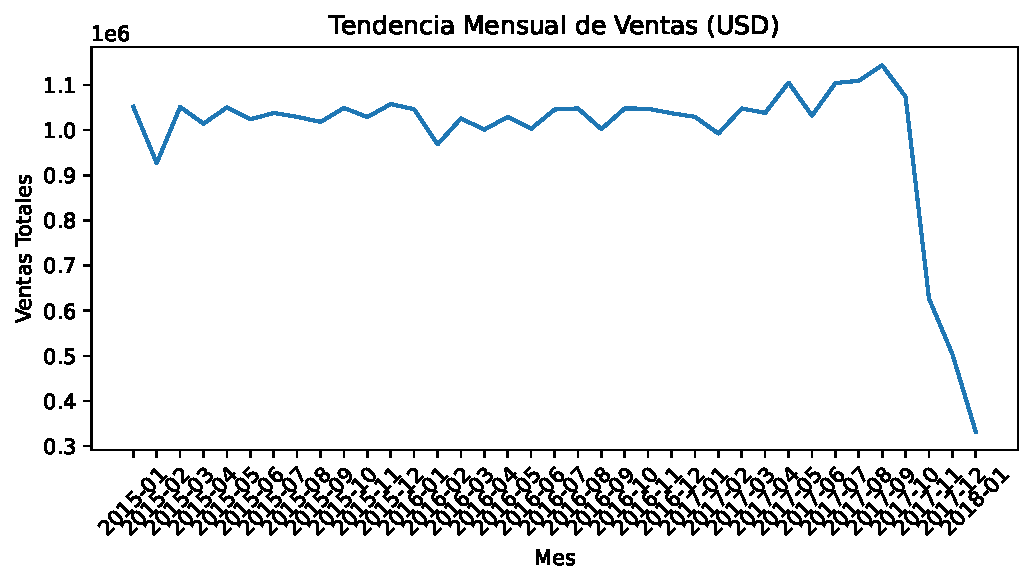
\includegraphics[keepaspectratio]{report_files/figure-pdf/temporal-analysis-output-1.pdf}}

\subsection{Distribución Geográfica y
Mercados}\label{distribuciuxf3n-geogruxe1fica-y-mercados}

DataCo opera en múltiples regiones. Europa y LATAM concentran la mayor
parte de las transacciones, pero también presentan retos logísticos
diferenciados.

\pandocbounded{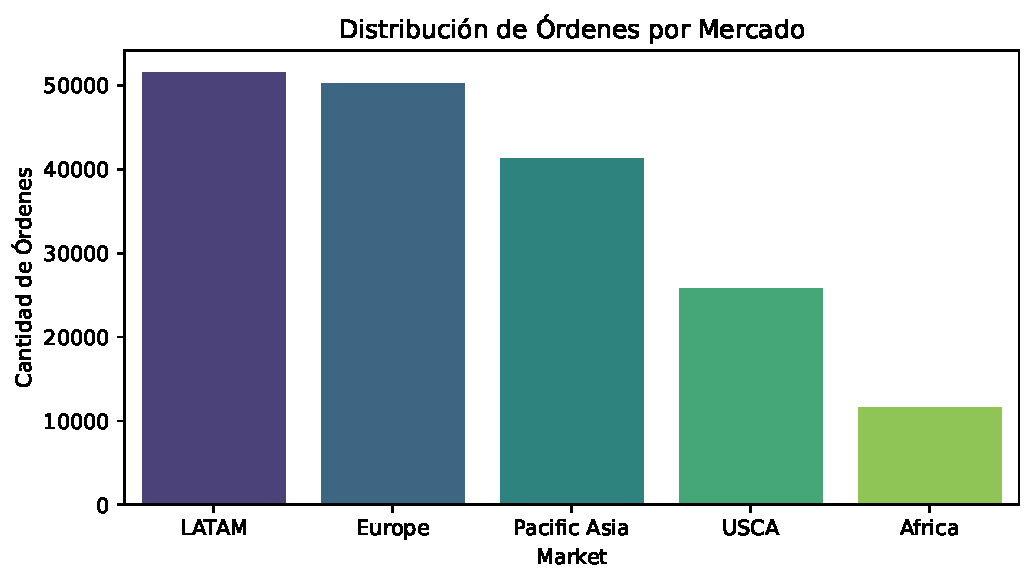
\includegraphics[keepaspectratio]{report_files/figure-pdf/geographic-analysis-output-1.pdf}}

\subsection{Distribución del Estado de
Entregas}\label{distribuciuxf3n-del-estado-de-entregas}

\protect\phantomsection\label{delivery-status}
\protect\phantomsection\label{delivery-status-1}
{\def\LTcaptype{none} % do not increment counter
\begin{longtable}[]{@{}ll@{}}
\toprule\noalign{}
& Proporción (\%) \\
Delivery Status & \\
\midrule\noalign{}
\endhead
\bottomrule\noalign{}
\endlastfoot
Late delivery & 54.83 \\
Advance shipping & 23.04 \\
Shipping on time & 17.84 \\
Shipping canceled & 4.30 \\
\end{longtable}
}

\pandocbounded{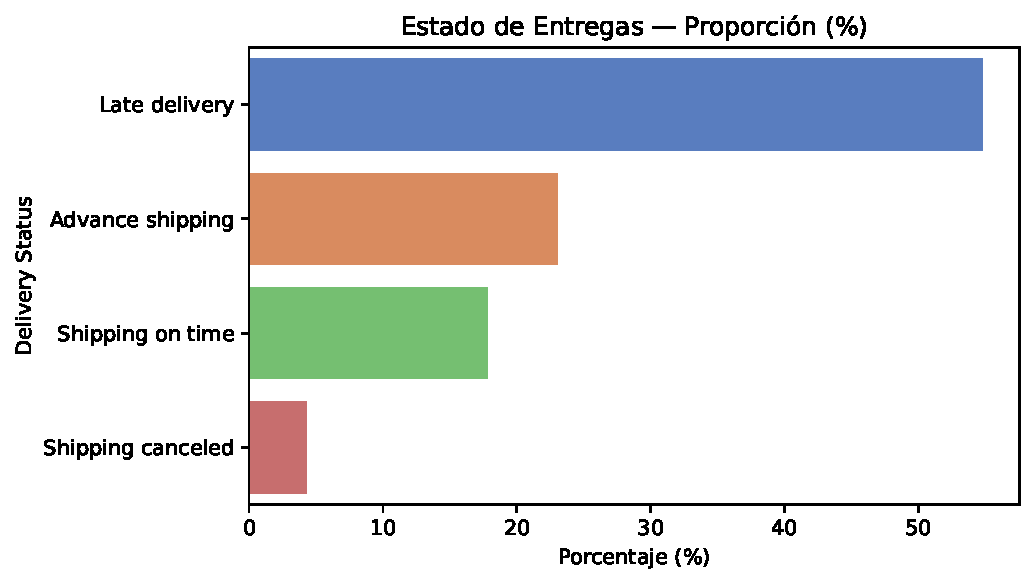
\includegraphics[keepaspectratio]{report_files/figure-pdf/delivery-status-output-2.pdf}}

El \textbf{54.8\%} de los envíos llega tarde, lo que confirma la
urgencia del problema y justifica la construcción de un modelo
predictivo.

\subsection{Distribuciones de Variables
Clave}\label{distribuciones-de-variables-clave}

\subsubsection{Tiempo Real de Envío}\label{tiempo-real-de-envuxedo}

\pandocbounded{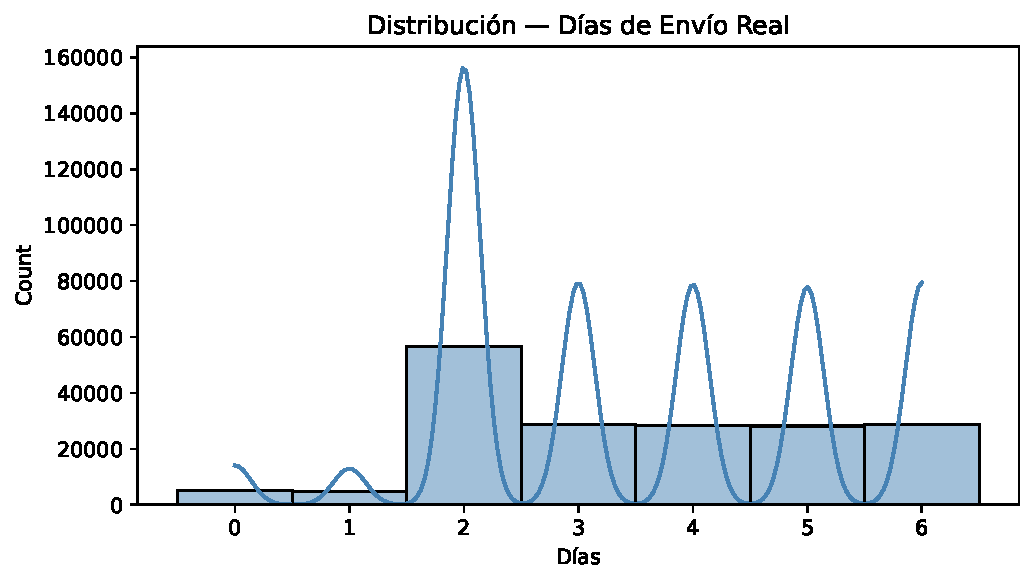
\includegraphics[keepaspectratio]{report_files/figure-pdf/dist-shipping-output-1.pdf}}

\subsubsection{Beneficio por Orden}\label{beneficio-por-orden}

\pandocbounded{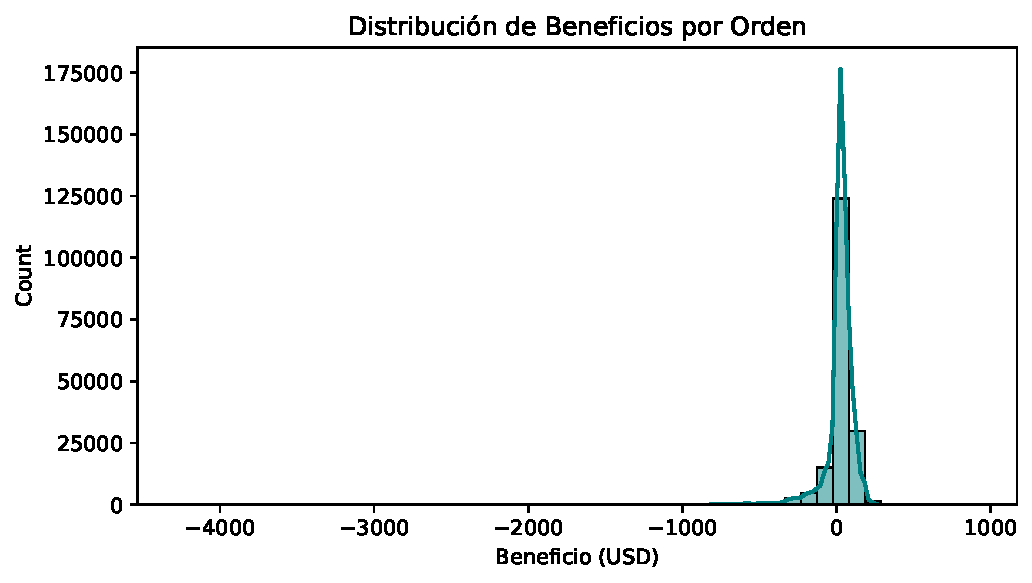
\includegraphics[keepaspectratio]{report_files/figure-pdf/benefit-dist-output-1.pdf}}

La cola izquierda confirma la existencia de una fracción significativa
de órdenes no rentables, crítica para la salud financiera de la
operación.

\subsection{Análisis Probabilístico y Teorema de
Bayes}\label{anuxe1lisis-probabiluxedstico-y-teorema-de-bayes}

Se definen tres eventos de interés para cuantificar escenarios críticos
de logística:

\begin{itemize}
\tightlist
\item
  \textbf{A}: Envío lento --- \texttt{Days\ for\ shipping\ (real)\ ≥\ 4}
\item
  \textbf{B}: Riesgo de retraso --- \texttt{Late\_delivery\_risk\ =\ 1}
\item
  \textbf{C}: Orden no rentable ---
  \texttt{Benefit\ per\ order\ ≤\ −100}
\end{itemize}

\subsubsection{Probabilidades Marginales y
Conjuntas}\label{probabilidades-marginales-y-conjuntas}

\protect\phantomsection\label{bayes-2var}
\begin{Shaded}
\begin{Highlighting}[]
\NormalTok{P\_A }\OperatorTok{=}\NormalTok{ (df[}\StringTok{"Days for shipping (real)"}\NormalTok{] }\OperatorTok{\textgreater{}=} \DecValTok{4}\NormalTok{).mean()}
\NormalTok{P\_B }\OperatorTok{=}\NormalTok{ (df[}\StringTok{"Late\_delivery\_risk"}\NormalTok{] }\OperatorTok{==} \DecValTok{1}\NormalTok{).mean()}
\NormalTok{P\_C }\OperatorTok{=}\NormalTok{ (df[}\StringTok{"Benefit per order"}\NormalTok{] }\OperatorTok{\textless{}=} \OperatorTok{{-}}\DecValTok{100}\NormalTok{).mean()}

\NormalTok{P\_AB  }\OperatorTok{=}\NormalTok{ ((df[}\StringTok{"Days for shipping (real)"}\NormalTok{] }\OperatorTok{\textgreater{}=} \DecValTok{4}\NormalTok{) }\OperatorTok{\&}\NormalTok{ (df[}\StringTok{"Late\_delivery\_risk"}\NormalTok{] }\OperatorTok{==} \DecValTok{1}\NormalTok{)).mean()}
\NormalTok{P\_AC  }\OperatorTok{=}\NormalTok{ ((df[}\StringTok{"Days for shipping (real)"}\NormalTok{] }\OperatorTok{\textgreater{}=} \DecValTok{4}\NormalTok{) }\OperatorTok{\&}\NormalTok{ (df[}\StringTok{"Benefit per order"}\NormalTok{] }\OperatorTok{\textless{}=} \OperatorTok{{-}}\DecValTok{100}\NormalTok{)).mean()}
\NormalTok{P\_BC  }\OperatorTok{=}\NormalTok{ ((df[}\StringTok{"Late\_delivery\_risk"}\NormalTok{] }\OperatorTok{==} \DecValTok{1}\NormalTok{) }\OperatorTok{\&}\NormalTok{ (df[}\StringTok{"Benefit per order"}\NormalTok{] }\OperatorTok{\textless{}=} \OperatorTok{{-}}\DecValTok{100}\NormalTok{)).mean()}
\NormalTok{P\_ABC }\OperatorTok{=}\NormalTok{ (}
\NormalTok{    (df[}\StringTok{"Days for shipping (real)"}\NormalTok{] }\OperatorTok{\textgreater{}=} \DecValTok{4}\NormalTok{) }\OperatorTok{\&}
\NormalTok{    (df[}\StringTok{"Late\_delivery\_risk"}\NormalTok{] }\OperatorTok{==} \DecValTok{1}\NormalTok{) }\OperatorTok{\&}
\NormalTok{    (df[}\StringTok{"Benefit per order"}\NormalTok{] }\OperatorTok{\textless{}=} \OperatorTok{{-}}\DecValTok{100}\NormalTok{)}
\NormalTok{).mean()}

\BuiltInTok{print}\NormalTok{(}\StringTok{"Probabilidades marginales:"}\NormalTok{)}
\BuiltInTok{print}\NormalTok{(}\SpecialStringTok{f"  P(A) Envío lento       = }\SpecialCharTok{\{}\NormalTok{P\_A}\SpecialCharTok{:.4f\}}\SpecialStringTok{  (}\SpecialCharTok{\{}\NormalTok{P\_A}\OperatorTok{*}\DecValTok{100}\SpecialCharTok{:.2f\}}\SpecialStringTok{\%)"}\NormalTok{)}
\BuiltInTok{print}\NormalTok{(}\SpecialStringTok{f"  P(B) Riesgo de retraso = }\SpecialCharTok{\{}\NormalTok{P\_B}\SpecialCharTok{:.4f\}}\SpecialStringTok{  (}\SpecialCharTok{\{}\NormalTok{P\_B}\OperatorTok{*}\DecValTok{100}\SpecialCharTok{:.2f\}}\SpecialStringTok{\%)"}\NormalTok{)}
\BuiltInTok{print}\NormalTok{(}\SpecialStringTok{f"  P(C) Orden no rentable = }\SpecialCharTok{\{}\NormalTok{P\_C}\SpecialCharTok{:.4f\}}\SpecialStringTok{  (}\SpecialCharTok{\{}\NormalTok{P\_C}\OperatorTok{*}\DecValTok{100}\SpecialCharTok{:.2f\}}\SpecialStringTok{\%)"}\NormalTok{)}

\BuiltInTok{print}\NormalTok{(}\StringTok{"}\CharTok{\textbackslash{}n}\StringTok{Probabilidades conjuntas:"}\NormalTok{)}
\BuiltInTok{print}\NormalTok{(}\SpecialStringTok{f"  P(A∩B)   = }\SpecialCharTok{\{}\NormalTok{P\_AB}\SpecialCharTok{:.4f\}}\SpecialStringTok{  (}\SpecialCharTok{\{}\NormalTok{P\_AB}\OperatorTok{*}\DecValTok{100}\SpecialCharTok{:.2f\}}\SpecialStringTok{\%)"}\NormalTok{)}
\BuiltInTok{print}\NormalTok{(}\SpecialStringTok{f"  P(A∩C)   = }\SpecialCharTok{\{}\NormalTok{P\_AC}\SpecialCharTok{:.4f\}}\SpecialStringTok{  (}\SpecialCharTok{\{}\NormalTok{P\_AC}\OperatorTok{*}\DecValTok{100}\SpecialCharTok{:.2f\}}\SpecialStringTok{\%)"}\NormalTok{)}
\BuiltInTok{print}\NormalTok{(}\SpecialStringTok{f"  P(B∩C)   = }\SpecialCharTok{\{}\NormalTok{P\_BC}\SpecialCharTok{:.4f\}}\SpecialStringTok{  (}\SpecialCharTok{\{}\NormalTok{P\_BC}\OperatorTok{*}\DecValTok{100}\SpecialCharTok{:.2f\}}\SpecialStringTok{\%)"}\NormalTok{)}
\BuiltInTok{print}\NormalTok{(}\SpecialStringTok{f"  P(A∩B∩C) = }\SpecialCharTok{\{}\NormalTok{P\_ABC}\SpecialCharTok{:.4f\}}\SpecialStringTok{  (}\SpecialCharTok{\{}\NormalTok{P\_ABC}\OperatorTok{*}\DecValTok{100}\SpecialCharTok{:.2f\}}\SpecialStringTok{\%)"}\NormalTok{)}
\end{Highlighting}
\end{Shaded}

\begin{verbatim}
Probabilidades marginales:
  P(A) Envío lento       = 0.4731  (47.31%)
  P(B) Riesgo de retraso = 0.5483  (54.83%)
  P(C) Orden no rentable = 0.0639  (6.39%)

Probabilidades conjuntas:
  P(A∩B)   = 0.3393  (33.93%)
  P(A∩C)   = 0.0306  (3.06%)
  P(B∩C)   = 0.0351  (3.51%)
  P(A∩B∩C) = 0.0221  (2.21%)
\end{verbatim}

\subsubsection{Probabilidades Condicionales vía
Bayes}\label{probabilidades-condicionales-vuxeda-bayes}

\protect\phantomsection\label{bayes-conditional}
\begin{Shaded}
\begin{Highlighting}[]
\NormalTok{P\_A\_dado\_B        }\OperatorTok{=}\NormalTok{ P\_AB }\OperatorTok{/}\NormalTok{ P\_B}
\NormalTok{P\_B\_dado\_A        }\OperatorTok{=}\NormalTok{ P\_AB }\OperatorTok{/}\NormalTok{ P\_A}
\NormalTok{P\_C\_dado\_A        }\OperatorTok{=}\NormalTok{ P\_AC }\OperatorTok{/}\NormalTok{ P\_A}
\NormalTok{P\_BC\_dado\_A       }\OperatorTok{=}\NormalTok{ P\_ABC }\OperatorTok{/}\NormalTok{ P\_A}
\NormalTok{P\_BC\_dado\_A\_bayes }\OperatorTok{=}\NormalTok{ (P\_ABC }\OperatorTok{/}\NormalTok{ P\_BC) }\OperatorTok{*}\NormalTok{ P\_BC }\OperatorTok{/}\NormalTok{ P\_A   }\CommentTok{\# verificación Bayes}

\BuiltInTok{print}\NormalTok{(}\StringTok{"Probabilidades condicionales:"}\NormalTok{)}
\BuiltInTok{print}\NormalTok{(}\SpecialStringTok{f"  P(B|A) = }\SpecialCharTok{\{}\NormalTok{P\_B\_dado\_A}\SpecialCharTok{:.4f\}}\SpecialStringTok{ (}\SpecialCharTok{\{}\NormalTok{P\_B\_dado\_A}\OperatorTok{*}\DecValTok{100}\SpecialCharTok{:.2f\}}\SpecialStringTok{\%) → Dado envío lento → riesgo de retraso"}\NormalTok{)}
\BuiltInTok{print}\NormalTok{(}\SpecialStringTok{f"  P(A|B) = }\SpecialCharTok{\{}\NormalTok{P\_A\_dado\_B}\SpecialCharTok{:.4f\}}\SpecialStringTok{ (}\SpecialCharTok{\{}\NormalTok{P\_A\_dado\_B}\OperatorTok{*}\DecValTok{100}\SpecialCharTok{:.2f\}}\SpecialStringTok{\%) → Dado retraso → envío fue lento"}\NormalTok{)}
\BuiltInTok{print}\NormalTok{(}\SpecialStringTok{f"  P(C|A) = }\SpecialCharTok{\{}\NormalTok{P\_C\_dado\_A}\SpecialCharTok{:.4f\}}\SpecialStringTok{ (}\SpecialCharTok{\{}\NormalTok{P\_C\_dado\_A}\OperatorTok{*}\DecValTok{100}\SpecialCharTok{:.2f\}}\SpecialStringTok{\%) → Dado envío lento → orden no rentable"}\NormalTok{)}
\BuiltInTok{print}\NormalTok{(}\SpecialStringTok{f"  P(B∩C|A) directo = }\SpecialCharTok{\{}\NormalTok{P\_BC\_dado\_A}\SpecialCharTok{:.4f\}}\SpecialStringTok{ (}\SpecialCharTok{\{}\NormalTok{P\_BC\_dado\_A}\OperatorTok{*}\DecValTok{100}\SpecialCharTok{:.2f\}}\SpecialStringTok{\%) → Envío lento → retraso Y pérdida"}\NormalTok{)}

\BuiltInTok{print}\NormalTok{(}\StringTok{"}\CharTok{\textbackslash{}n}\StringTok{Verificación independencia (A y C):"}\NormalTok{)}
\BuiltInTok{print}\NormalTok{(}\SpecialStringTok{f"  P(A)·P(C) = }\SpecialCharTok{\{}\NormalTok{P\_A}\OperatorTok{*}\NormalTok{P\_C}\SpecialCharTok{:.4f\}}\SpecialStringTok{  vs  P(A∩C) = }\SpecialCharTok{\{}\NormalTok{P\_AC}\SpecialCharTok{:.4f\}}\SpecialStringTok{"}\NormalTok{)}
\ControlFlowTok{if} \BuiltInTok{abs}\NormalTok{(P\_A }\OperatorTok{*}\NormalTok{ P\_C }\OperatorTok{{-}}\NormalTok{ P\_AC) }\OperatorTok{\textless{}} \FloatTok{0.001}\NormalTok{:}
    \BuiltInTok{print}\NormalTok{(}\StringTok{"  → Eventos aproximadamente INDEPENDIENTES"}\NormalTok{)}
\ControlFlowTok{else}\NormalTok{:}
    \BuiltInTok{print}\NormalTok{(}\StringTok{"  → Eventos NO independientes (hay asociación)"}\NormalTok{)}
\end{Highlighting}
\end{Shaded}

\begin{verbatim}
Probabilidades condicionales:
  P(B|A) = 0.7172 (71.72%) → Dado envío lento → riesgo de retraso
  P(A|B) = 0.6188 (61.88%) → Dado retraso → envío fue lento
  P(C|A) = 0.0648 (6.48%) → Dado envío lento → orden no rentable
  P(B∩C|A) directo = 0.0467 (4.67%) → Envío lento → retraso Y pérdida

Verificación independencia (A y C):
  P(A)·P(C) = 0.0302  vs  P(A∩C) = 0.0306
  → Eventos aproximadamente INDEPENDIENTES
\end{verbatim}

El análisis confirma que el envío lento es un predictor fuerte del
riesgo de retraso: dado un envío con \texttt{Days\ ≥\ 4}, la
probabilidad de entrega tardía asciende al \textbf{71.7\%}.

\subsection{Muestreo Aleatorio e Intervalo de
Confianza}\label{muestreo-aleatorio-e-intervalo-de-confianza}

Para validar la representatividad de una muestra, se aplica muestreo
aleatorio simple (5\%) y se construye un intervalo de confianza al 95\%
para la variable \texttt{Sales\ per\ customer}.

\protect\phantomsection\label{sampling-ci}
\begin{Shaded}
\begin{Highlighting}[]
\NormalTok{df\_muestra }\OperatorTok{=}\NormalTok{ df.sample(frac}\OperatorTok{=}\FloatTok{0.05}\NormalTok{, random\_state}\OperatorTok{=}\DecValTok{42}\NormalTok{)}

\NormalTok{col }\OperatorTok{=} \StringTok{\textquotesingle{}Sales per customer\textquotesingle{}}
\NormalTok{media }\OperatorTok{=}\NormalTok{ df\_muestra[col].mean()}
\NormalTok{std   }\OperatorTok{=}\NormalTok{ df\_muestra[col].std()}
\NormalTok{n     }\OperatorTok{=} \BuiltInTok{len}\NormalTok{(df\_muestra)}

\NormalTok{SE    }\OperatorTok{=}\NormalTok{ std }\OperatorTok{/}\NormalTok{ np.sqrt(n)}
\NormalTok{Z     }\OperatorTok{=} \FloatTok{1.96}
\NormalTok{error }\OperatorTok{=}\NormalTok{ SE }\OperatorTok{*}\NormalTok{ Z}

\NormalTok{IC\_L }\OperatorTok{=}\NormalTok{ media }\OperatorTok{{-}}\NormalTok{ error}
\NormalTok{IC\_U }\OperatorTok{=}\NormalTok{ media }\OperatorTok{+}\NormalTok{ error}

\BuiltInTok{print}\NormalTok{(}\SpecialStringTok{f"Muestra: n = }\SpecialCharTok{\{}\NormalTok{n}\SpecialCharTok{:,\}}\SpecialStringTok{ (}\SpecialCharTok{\{}\NormalTok{n}\OperatorTok{/}\BuiltInTok{len}\NormalTok{(df)}\OperatorTok{*}\DecValTok{100}\SpecialCharTok{:.0f\}}\SpecialStringTok{\% del total)"}\NormalTok{)}
\BuiltInTok{print}\NormalTok{(}\SpecialStringTok{f"Media muestral de \textquotesingle{}}\SpecialCharTok{\{}\NormalTok{col}\SpecialCharTok{\}}\SpecialStringTok{\textquotesingle{}: }\SpecialCharTok{\{}\NormalTok{media}\SpecialCharTok{:.2f\}}\SpecialStringTok{ USD"}\NormalTok{)}
\BuiltInTok{print}\NormalTok{(}\SpecialStringTok{f"Desviación estándar: }\SpecialCharTok{\{}\NormalTok{std}\SpecialCharTok{:.2f\}}\SpecialStringTok{"}\NormalTok{)}
\BuiltInTok{print}\NormalTok{(}\SpecialStringTok{f"Error estándar (SE): }\SpecialCharTok{\{}\NormalTok{SE}\SpecialCharTok{:.4f\}}\SpecialStringTok{"}\NormalTok{)}
\BuiltInTok{print}\NormalTok{(}\SpecialStringTok{f"Intervalo de confianza 95\%: [}\SpecialCharTok{\{}\NormalTok{IC\_L}\SpecialCharTok{:.2f\}}\SpecialStringTok{, }\SpecialCharTok{\{}\NormalTok{IC\_U}\SpecialCharTok{:.2f\}}\SpecialStringTok{] USD"}\NormalTok{)}
\end{Highlighting}
\end{Shaded}

\begin{verbatim}
Muestra: n = 9,026 (5% del total)
Media muestral de 'Sales per customer': 184.39 USD
Desviación estándar: 120.41
Error estándar (SE): 1.2674
Intervalo de confianza 95%: [181.91, 186.88] USD
\end{verbatim}

\subsection{Matriz de Correlación}\label{matriz-de-correlaciuxf3n}

\protect\phantomsection\label{correlation-matrix}
\pandocbounded{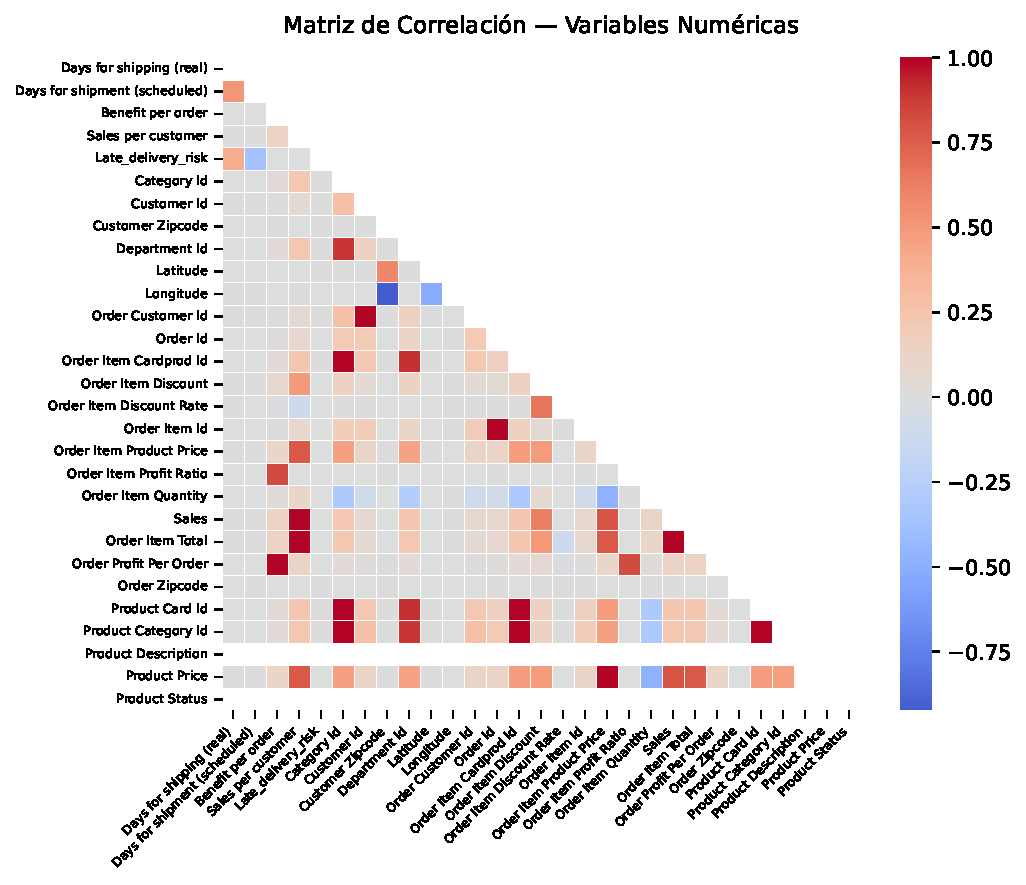
\includegraphics[keepaspectratio]{report_files/figure-pdf/correlation-matrix-output-1.pdf}}

\begin{verbatim}

Correlaciones con Late_delivery_risk (por valor absoluto):
\end{verbatim}

\protect\phantomsection\label{correlation-matrix-2}
{\def\LTcaptype{none} % do not increment counter
\begin{longtable}[]{@{}ll@{}}
\toprule\noalign{}
& Correlación \\
\midrule\noalign{}
\endhead
\bottomrule\noalign{}
\endlastfoot
Days for shipping (real) & 0.401415 \\
Days for shipment (scheduled) & -0.369352 \\
Order Zipcode & -0.014131 \\
Sales per customer & -0.003791 \\
Order Item Total & -0.003791 \\
Order Profit Per Order & -0.003727 \\
Benefit per order & -0.003727 \\
Sales & -0.003564 \\
\end{longtable}
}

\section{Definición del Problema y
Metodología}\label{definiciuxf3n-del-problema-y-metodologuxeda}

\subsection{Selección del Problema: Late Delivery
Risk}\label{selecciuxf3n-del-problema-late-delivery-risk}

En la logística moderna, el cumplimiento de los tiempos de entrega es el
factor crítico de la satisfacción del cliente. DataCo define el
\textbf{Riesgo de Entrega Tardía} (\texttt{Late\_delivery\_risk}) como
un indicador binario activo cuando el tiempo real de envío supera al
tiempo programado.

Dado que el \textasciitilde55\% de las órdenes presenta este riesgo, su
predicción temprana permite:

\begin{itemize}
\tightlist
\item
  Notificar proactivamente al cliente.
\item
  Reasignar transportistas en rutas críticas.
\item
  Optimizar la planificación de inventarios regionales.
\end{itemize}

\subsection{Preprocesamiento y Prevención de Data
Leakage}\label{preprocesamiento-y-prevenciuxf3n-de-data-leakage}

Se aplicaron las siguientes transformaciones en todos los pipelines de
modelado:

\begin{enumerate}
\def\labelenumi{\arabic{enumi}.}
\tightlist
\item
  \textbf{Imputación de valores nulos} mediante la mediana
  (\texttt{SimpleImputer(strategy="median")}).
\item
  \textbf{Normalización} con \texttt{StandardScaler} para evitar que las
  magnitudes afecten a los modelos lineales.
\item
  \textbf{Eliminación de variables con fuga de datos} --- columnas que
  revelan información post-evento no disponible al momento del despacho:

  \begin{itemize}
  \tightlist
  \item
    \texttt{Delivery\ Status} (resultado conocido después del hecho).
  \item
    \texttt{Days\ for\ shipping\ (real)} (componente directo del cálculo
    del riesgo de clasificación).
  \item
    Variables financieras derivadas de \texttt{Sales} para el modelo de
    regresión.
  \end{itemize}
\end{enumerate}

\section{Implementación y Evaluación de
Modelos}\label{implementaciuxf3n-y-evaluaciuxf3n-de-modelos}

El modelado se abordó desde dos perspectivas: regresión (predicción de
ventas totales) y clasificación (predicción del riesgo de entrega
tardía).

\subsection{Modelo de Regresión: Predicción de
Ventas}\label{modelo-de-regresiuxf3n-predicciuxf3n-de-ventas}

Benchmarking de cuatro modelos lineales para estimar \texttt{Sales} a
partir de variables numéricas del pedido.

\begin{Shaded}
\begin{Highlighting}[]
\ImportTok{import}\NormalTok{ time}

\ImportTok{from}\NormalTok{ sklearn.impute }\ImportTok{import}\NormalTok{ SimpleImputer}
\ImportTok{from}\NormalTok{ sklearn.linear\_model }\ImportTok{import}\NormalTok{ ElasticNet, Lasso, LinearRegression, Ridge}
\ImportTok{from}\NormalTok{ sklearn.metrics }\ImportTok{import}\NormalTok{ mean\_absolute\_error, r2\_score, root\_mean\_squared\_error}
\ImportTok{from}\NormalTok{ sklearn.model\_selection }\ImportTok{import}\NormalTok{ train\_test\_split}
\ImportTok{from}\NormalTok{ sklearn.pipeline }\ImportTok{import}\NormalTok{ Pipeline}
\ImportTok{from}\NormalTok{ sklearn.preprocessing }\ImportTok{import}\NormalTok{ StandardScaler}

\NormalTok{TARGET }\OperatorTok{=} \StringTok{\textquotesingle{}Sales\textquotesingle{}}

\NormalTok{drop\_cols }\OperatorTok{=}\NormalTok{ [}
\NormalTok{    TARGET,}
    \StringTok{\textquotesingle{}Customer Id\textquotesingle{}}\NormalTok{, }\StringTok{\textquotesingle{}Order Customer Id\textquotesingle{}}\NormalTok{, }\StringTok{\textquotesingle{}Order Id\textquotesingle{}}\NormalTok{,}
    \StringTok{\textquotesingle{}Order Item Id\textquotesingle{}}\NormalTok{, }\StringTok{\textquotesingle{}Order Item Cardprod Id\textquotesingle{}}\NormalTok{,}
    \StringTok{\textquotesingle{}Product Card Id\textquotesingle{}}\NormalTok{, }\StringTok{\textquotesingle{}Product Category Id\textquotesingle{}}\NormalTok{, }\StringTok{\textquotesingle{}Category Id\textquotesingle{}}\NormalTok{, }\StringTok{\textquotesingle{}Department Id\textquotesingle{}}\NormalTok{,}
    \CommentTok{\# Fuga de datos — derivadas de Sales}
    \StringTok{\textquotesingle{}Order Item Total\textquotesingle{}}\NormalTok{,}
    \StringTok{\textquotesingle{}Order Profit Per Order\textquotesingle{}}\NormalTok{,}
    \StringTok{\textquotesingle{}Benefit per order\textquotesingle{}}\NormalTok{,}
    \CommentTok{\# Sin datos útiles}
    \StringTok{\textquotesingle{}Product Description\textquotesingle{}}\NormalTok{,}
\NormalTok{]}

\NormalTok{numeric\_cols }\OperatorTok{=}\NormalTok{ df.select\_dtypes(include}\OperatorTok{=}\NormalTok{[np.number]).columns.tolist()}
\NormalTok{feature\_cols }\OperatorTok{=}\NormalTok{ [c }\ControlFlowTok{for}\NormalTok{ c }\KeywordTok{in}\NormalTok{ numeric\_cols }\ControlFlowTok{if}\NormalTok{ c }\KeywordTok{not} \KeywordTok{in}\NormalTok{ drop\_cols]}

\NormalTok{X }\OperatorTok{=}\NormalTok{ df[feature\_cols]}
\NormalTok{y }\OperatorTok{=}\NormalTok{ df[TARGET]}

\NormalTok{X\_train, X\_test, y\_train, y\_test }\OperatorTok{=}\NormalTok{ train\_test\_split(X, y, test\_size}\OperatorTok{=}\FloatTok{0.2}\NormalTok{, random\_state}\OperatorTok{=}\DecValTok{42}\NormalTok{)}

\NormalTok{models\_reg }\OperatorTok{=}\NormalTok{ \{}
    \StringTok{"Linear Regression"}\NormalTok{: LinearRegression(),}
    \StringTok{"Ridge"}\NormalTok{:             Ridge(alpha}\OperatorTok{=}\FloatTok{1.0}\NormalTok{),}
    \StringTok{"Lasso"}\NormalTok{:             Lasso(alpha}\OperatorTok{=}\FloatTok{1.0}\NormalTok{, max\_iter}\OperatorTok{=}\DecValTok{5000}\NormalTok{),}
    \StringTok{"ElasticNet"}\NormalTok{:        ElasticNet(alpha}\OperatorTok{=}\FloatTok{1.0}\NormalTok{, l1\_ratio}\OperatorTok{=}\FloatTok{0.5}\NormalTok{, max\_iter}\OperatorTok{=}\DecValTok{5000}\NormalTok{),}
\NormalTok{\}}

\NormalTok{results\_reg }\OperatorTok{=}\NormalTok{ []}

\ControlFlowTok{for}\NormalTok{ name, model }\KeywordTok{in}\NormalTok{ models\_reg.items():}
\NormalTok{    pipe }\OperatorTok{=}\NormalTok{ Pipeline([}
\NormalTok{        (}\StringTok{"imputer"}\NormalTok{, SimpleImputer(strategy}\OperatorTok{=}\StringTok{"median"}\NormalTok{)),}
\NormalTok{        (}\StringTok{"scaler"}\NormalTok{,  StandardScaler()),}
\NormalTok{        (}\StringTok{"model"}\NormalTok{,   model),}
\NormalTok{    ])}
\NormalTok{    start }\OperatorTok{=}\NormalTok{ time.time()}
\NormalTok{    pipe.fit(X\_train, y\_train)}
\NormalTok{    elapsed }\OperatorTok{=}\NormalTok{ time.time() }\OperatorTok{{-}}\NormalTok{ start}
\NormalTok{    y\_pred }\OperatorTok{=}\NormalTok{ pipe.predict(X\_test)}
\NormalTok{    results\_reg.append(\{}
        \StringTok{"Modelo"}\NormalTok{:    name,}
        \StringTok{"MAE"}\NormalTok{:       }\BuiltInTok{round}\NormalTok{(mean\_absolute\_error(y\_test, y\_pred), }\DecValTok{4}\NormalTok{),}
        \StringTok{"RMSE"}\NormalTok{:      }\BuiltInTok{round}\NormalTok{(root\_mean\_squared\_error(y\_test, y\_pred), }\DecValTok{4}\NormalTok{),}
        \StringTok{"R²"}\NormalTok{:        }\BuiltInTok{round}\NormalTok{(r2\_score(y\_test, y\_pred), }\DecValTok{4}\NormalTok{),}
        \StringTok{"Tiempo(s)"}\NormalTok{: }\BuiltInTok{round}\NormalTok{(elapsed, }\DecValTok{4}\NormalTok{),}
\NormalTok{    \})}

\NormalTok{results\_reg\_df }\OperatorTok{=}\NormalTok{ pd.DataFrame(results\_reg).set\_index(}\StringTok{"Modelo"}\NormalTok{).sort\_values(}\StringTok{"R²"}\NormalTok{, ascending}\OperatorTok{=}\VariableTok{False}\NormalTok{)}
\BuiltInTok{print}\NormalTok{(}\SpecialStringTok{f"}\CharTok{\textbackslash{}u2705}\SpecialStringTok{ Mejor modelo por R²: }\SpecialCharTok{\{}\NormalTok{results\_reg\_df[}\StringTok{\textquotesingle{}R²\textquotesingle{}}\NormalTok{]}\SpecialCharTok{.}\NormalTok{idxmax()}\SpecialCharTok{\}}\SpecialStringTok{"}\NormalTok{)}
\NormalTok{display(results\_reg\_df.style.}\BuiltInTok{format}\NormalTok{(}\StringTok{"}\SpecialCharTok{\{:.4f\}}\StringTok{"}\NormalTok{).set\_caption(}\StringTok{"Benchmarking — Modelos de Regresión"}\NormalTok{))}
\end{Highlighting}
\end{Shaded}

\begin{verbatim}
✅ Mejor modelo por R²: Linear Regression
\end{verbatim}

\protect\phantomsection\label{regression-model}
\begin{longtable}[]{@{}lllll@{}}
\caption{Benchmarking --- Modelos de
Regresión}\label{T_a6051}\tabularnewline
\toprule\noalign{}
~ & MAE & RMSE & R² & Tiempo(s) \\
Modelo & ~ & ~ & ~ & ~ \\
\midrule\noalign{}
\endfirsthead
\toprule\noalign{}
~ & MAE & RMSE & R² & Tiempo(s) \\
Modelo & ~ & ~ & ~ & ~ \\
\midrule\noalign{}
\endhead
\bottomrule\noalign{}
\endlastfoot
Linear Regression & 0.0006 & 0.0015 & 1.0000 & 0.3566 \\
Ridge & 0.0017 & 0.0033 & 1.0000 & 0.2355 \\
Lasso & 0.8359 & 1.1550 & 0.9999 & 1.3566 \\
ElasticNet & 21.3449 & 30.1334 & 0.9476 & 0.7855 \\
\end{longtable}

\subsection{Modelo de Clasificación: Riesgo de Entrega
Tardía}\label{modelo-de-clasificaciuxf3n-riesgo-de-entrega-tarduxeda}

\subsubsection{Paso 1 --- Selección de Features por
Importancia}\label{paso-1-selecciuxf3n-de-features-por-importancia}

Se usa un Decision Tree de referencia para filtrar variables con
importancia ≥ 1\%.

\protect\phantomsection\label{clf-feature-selection}
\begin{Shaded}
\begin{Highlighting}[]
\ImportTok{from}\NormalTok{ sklearn.metrics }\ImportTok{import}\NormalTok{ accuracy\_score, classification\_report}
\ImportTok{from}\NormalTok{ sklearn.tree }\ImportTok{import}\NormalTok{ DecisionTreeClassifier}

\NormalTok{TARGET\_CLF }\OperatorTok{=} \StringTok{\textquotesingle{}Late\_delivery\_risk\textquotesingle{}}

\NormalTok{drop\_cols\_clf }\OperatorTok{=}\NormalTok{ [}
\NormalTok{    TARGET\_CLF,}
    \StringTok{\textquotesingle{}Customer Id\textquotesingle{}}\NormalTok{, }\StringTok{\textquotesingle{}Order Customer Id\textquotesingle{}}\NormalTok{, }\StringTok{\textquotesingle{}Order Id\textquotesingle{}}\NormalTok{,}
    \StringTok{\textquotesingle{}Order Item Id\textquotesingle{}}\NormalTok{, }\StringTok{\textquotesingle{}Order Item Cardprod Id\textquotesingle{}}\NormalTok{,}
    \StringTok{\textquotesingle{}Product Card Id\textquotesingle{}}\NormalTok{, }\StringTok{\textquotesingle{}Product Category Id\textquotesingle{}}\NormalTok{, }\StringTok{\textquotesingle{}Category Id\textquotesingle{}}\NormalTok{, }\StringTok{\textquotesingle{}Department Id\textquotesingle{}}\NormalTok{,}
    \StringTok{\textquotesingle{}Product Description\textquotesingle{}}\NormalTok{,}
\NormalTok{]}

\NormalTok{numeric\_cols\_clf }\OperatorTok{=}\NormalTok{ df.select\_dtypes(include}\OperatorTok{=}\NormalTok{[np.number]).columns.tolist()}
\NormalTok{feature\_cols\_clf }\OperatorTok{=}\NormalTok{ [c }\ControlFlowTok{for}\NormalTok{ c }\KeywordTok{in}\NormalTok{ numeric\_cols\_clf }\ControlFlowTok{if}\NormalTok{ c }\KeywordTok{not} \KeywordTok{in}\NormalTok{ drop\_cols\_clf]}

\NormalTok{X\_clf }\OperatorTok{=}\NormalTok{ df[feature\_cols\_clf]}
\NormalTok{y\_clf }\OperatorTok{=}\NormalTok{ df[TARGET\_CLF]}

\NormalTok{X\_train\_clf, X\_test\_clf, y\_train\_clf, y\_test\_clf }\OperatorTok{=}\NormalTok{ train\_test\_split(}
\NormalTok{    X\_clf, y\_clf, test\_size}\OperatorTok{=}\FloatTok{0.2}\NormalTok{, random\_state}\OperatorTok{=}\DecValTok{42}\NormalTok{, stratify}\OperatorTok{=}\NormalTok{y\_clf}
\NormalTok{)}

\NormalTok{dt\_ref }\OperatorTok{=}\NormalTok{ Pipeline([}
\NormalTok{    (}\StringTok{"imputer"}\NormalTok{, SimpleImputer(strategy}\OperatorTok{=}\StringTok{"median"}\NormalTok{)),}
\NormalTok{    (}\StringTok{"scaler"}\NormalTok{,  StandardScaler()),}
\NormalTok{    (}\StringTok{"model"}\NormalTok{,   DecisionTreeClassifier(max\_depth}\OperatorTok{=}\DecValTok{6}\NormalTok{, random\_state}\OperatorTok{=}\DecValTok{42}\NormalTok{)),}
\NormalTok{])}
\NormalTok{dt\_ref.fit(X\_train\_clf, y\_train\_clf)}

\NormalTok{importances }\OperatorTok{=}\NormalTok{ pd.Series(}
\NormalTok{    dt\_ref.named\_steps[}\StringTok{"model"}\NormalTok{].feature\_importances\_,}
\NormalTok{    index}\OperatorTok{=}\NormalTok{feature\_cols\_clf}
\NormalTok{).sort\_values(ascending}\OperatorTok{=}\VariableTok{False}\NormalTok{)}

\NormalTok{IMPORTANCE\_THRESHOLD }\OperatorTok{=} \FloatTok{0.01}
\NormalTok{selected\_features }\OperatorTok{=}\NormalTok{ importances[importances }\OperatorTok{\textgreater{}=}\NormalTok{ IMPORTANCE\_THRESHOLD].index.tolist()}

\BuiltInTok{print}\NormalTok{(}\SpecialStringTok{f"Features seleccionadas (}\SpecialCharTok{\{}\BuiltInTok{len}\NormalTok{(selected\_features)}\SpecialCharTok{\}}\SpecialStringTok{):"}\NormalTok{)}
\ControlFlowTok{for}\NormalTok{ feat }\KeywordTok{in}\NormalTok{ selected\_features:}
    \BuiltInTok{print}\NormalTok{(}\SpecialStringTok{f"  }\SpecialCharTok{\{}\NormalTok{feat}\SpecialCharTok{:\textless{}35\}}\SpecialStringTok{ }\SpecialCharTok{\{}\NormalTok{importances[feat]}\SpecialCharTok{:.4f\}}\SpecialStringTok{"}\NormalTok{)}

\NormalTok{X\_final }\OperatorTok{=}\NormalTok{ df[selected\_features]}
\NormalTok{y\_final }\OperatorTok{=}\NormalTok{ df[TARGET\_CLF]}

\NormalTok{X\_train\_f, X\_test\_f, y\_train\_f, y\_test\_f }\OperatorTok{=}\NormalTok{ train\_test\_split(}
\NormalTok{    X\_final, y\_final, test\_size}\OperatorTok{=}\FloatTok{0.2}\NormalTok{, random\_state}\OperatorTok{=}\DecValTok{42}\NormalTok{, stratify}\OperatorTok{=}\NormalTok{y\_final}
\NormalTok{)}
\BuiltInTok{print}\NormalTok{(}\SpecialStringTok{f"}\CharTok{\textbackslash{}n}\SpecialStringTok{Entrenamiento: X=}\SpecialCharTok{\{}\NormalTok{X\_train\_f}\SpecialCharTok{.}\NormalTok{shape}\SpecialCharTok{\}}\SpecialStringTok{ | y=}\SpecialCharTok{\{}\NormalTok{y\_train\_f}\SpecialCharTok{.}\NormalTok{shape}\SpecialCharTok{\}}\SpecialStringTok{"}\NormalTok{)}
\BuiltInTok{print}\NormalTok{(}\SpecialStringTok{f"Prueba       : X=}\SpecialCharTok{\{}\NormalTok{X\_test\_f}\SpecialCharTok{.}\NormalTok{shape}\SpecialCharTok{\}}\SpecialStringTok{  | y=}\SpecialCharTok{\{}\NormalTok{y\_test\_f}\SpecialCharTok{.}\NormalTok{shape}\SpecialCharTok{\}}\SpecialStringTok{"}\NormalTok{)}
\end{Highlighting}
\end{Shaded}

\begin{verbatim}
Features seleccionadas (2):
  Days for shipping (real)            0.5323
  Days for shipment (scheduled)       0.4670

Entrenamiento: X=(144415, 2) | y=(144415,)
Prueba       : X=(36104, 2)  | y=(36104,)
\end{verbatim}

\subsubsection{Paso 2 --- Benchmarking de
Clasificadores}\label{paso-2-benchmarking-de-clasificadores}

\begin{Shaded}
\begin{Highlighting}[]
\ImportTok{from}\NormalTok{ sklearn.ensemble }\ImportTok{import}\NormalTok{ RandomForestClassifier}
\ImportTok{from}\NormalTok{ sklearn.linear\_model }\ImportTok{import}\NormalTok{ LogisticRegression}
\ImportTok{from}\NormalTok{ sklearn.metrics }\ImportTok{import}\NormalTok{ (}
\NormalTok{    accuracy\_score, f1\_score, precision\_score, recall\_score, roc\_auc\_score,}
\NormalTok{)}
\ImportTok{from}\NormalTok{ xgboost }\ImportTok{import}\NormalTok{ XGBClassifier}

\NormalTok{clf\_models }\OperatorTok{=}\NormalTok{ \{}
    \StringTok{"Logistic Regression"}\NormalTok{: LogisticRegression(max\_iter}\OperatorTok{=}\DecValTok{1000}\NormalTok{, random\_state}\OperatorTok{=}\DecValTok{42}\NormalTok{),}
    \StringTok{"Decision Tree"}\NormalTok{:       DecisionTreeClassifier(max\_depth}\OperatorTok{=}\DecValTok{6}\NormalTok{, random\_state}\OperatorTok{=}\DecValTok{42}\NormalTok{),}
    \StringTok{"Random Forest"}\NormalTok{:       RandomForestClassifier(n\_estimators}\OperatorTok{=}\DecValTok{100}\NormalTok{, max\_depth}\OperatorTok{=}\DecValTok{6}\NormalTok{,}
\NormalTok{                                                  random\_state}\OperatorTok{=}\DecValTok{42}\NormalTok{, n\_jobs}\OperatorTok{={-}}\DecValTok{1}\NormalTok{),}
    \StringTok{"XGBoost"}\NormalTok{:             XGBClassifier(n\_estimators}\OperatorTok{=}\DecValTok{100}\NormalTok{, max\_depth}\OperatorTok{=}\DecValTok{6}\NormalTok{,}
\NormalTok{                                         learning\_rate}\OperatorTok{=}\FloatTok{0.1}\NormalTok{, random\_state}\OperatorTok{=}\DecValTok{42}\NormalTok{,}
\NormalTok{                                         eval\_metric}\OperatorTok{=}\StringTok{"logloss"}\NormalTok{,}
\NormalTok{                                         verbosity}\OperatorTok{=}\DecValTok{0}\NormalTok{),}
\NormalTok{\}}

\NormalTok{clf\_results }\OperatorTok{=}\NormalTok{ []}

\ControlFlowTok{for}\NormalTok{ name, model }\KeywordTok{in}\NormalTok{ clf\_models.items():}
\NormalTok{    pipe }\OperatorTok{=}\NormalTok{ Pipeline([}
\NormalTok{        (}\StringTok{"imputer"}\NormalTok{, SimpleImputer(strategy}\OperatorTok{=}\StringTok{"median"}\NormalTok{)),}
\NormalTok{        (}\StringTok{"scaler"}\NormalTok{,  StandardScaler()),}
\NormalTok{        (}\StringTok{"model"}\NormalTok{,   model),}
\NormalTok{    ])}
\NormalTok{    start }\OperatorTok{=}\NormalTok{ time.time()}
\NormalTok{    pipe.fit(X\_train\_f, y\_train\_f)}
\NormalTok{    elapsed }\OperatorTok{=}\NormalTok{ time.time() }\OperatorTok{{-}}\NormalTok{ start}

\NormalTok{    y\_pred  }\OperatorTok{=}\NormalTok{ pipe.predict(X\_test\_f)}
\NormalTok{    y\_proba }\OperatorTok{=}\NormalTok{ pipe.predict\_proba(X\_test\_f)[:, }\DecValTok{1}\NormalTok{]}

\NormalTok{    clf\_results.append(\{}
        \StringTok{"Modelo"}\NormalTok{:    name,}
        \StringTok{"Accuracy"}\NormalTok{:  accuracy\_score(y\_test\_f, y\_pred),}
        \StringTok{"Precision"}\NormalTok{: precision\_score(y\_test\_f, y\_pred, zero\_division}\OperatorTok{=}\DecValTok{0}\NormalTok{),}
        \StringTok{"Recall"}\NormalTok{:    recall\_score(y\_test\_f, y\_pred, zero\_division}\OperatorTok{=}\DecValTok{0}\NormalTok{),}
        \StringTok{"F1{-}Score"}\NormalTok{:  f1\_score(y\_test\_f, y\_pred, zero\_division}\OperatorTok{=}\DecValTok{0}\NormalTok{),}
        \StringTok{"ROC{-}AUC"}\NormalTok{:   roc\_auc\_score(y\_test\_f, y\_proba),}
        \StringTok{"Tiempo(s)"}\NormalTok{: }\BuiltInTok{round}\NormalTok{(elapsed, }\DecValTok{4}\NormalTok{),}
\NormalTok{    \})}
    \BuiltInTok{print}\NormalTok{(}\SpecialStringTok{f"✔ }\SpecialCharTok{\{}\NormalTok{name}\SpecialCharTok{:\textless{}22\}}\SpecialStringTok{ entrenado en }\SpecialCharTok{\{}\NormalTok{elapsed}\SpecialCharTok{:.4f\}}\SpecialStringTok{s"}\NormalTok{)}

\NormalTok{clf\_results\_df }\OperatorTok{=}\NormalTok{ pd.DataFrame(clf\_results).set\_index(}\StringTok{"Modelo"}\NormalTok{).sort\_values(}\StringTok{"F1{-}Score"}\NormalTok{, ascending}\OperatorTok{=}\VariableTok{False}\NormalTok{)}

\BuiltInTok{print}\NormalTok{(}\SpecialStringTok{f"🏆 Mejor Accuracy : }\SpecialCharTok{\{}\NormalTok{clf\_results\_df[}\StringTok{\textquotesingle{}Accuracy\textquotesingle{}}\NormalTok{]}\SpecialCharTok{.}\NormalTok{idxmax()}\SpecialCharTok{\}}\SpecialStringTok{"}\NormalTok{)}
\BuiltInTok{print}\NormalTok{(}\SpecialStringTok{f"🏆 Mejor F1{-}Score : }\SpecialCharTok{\{}\NormalTok{clf\_results\_df[}\StringTok{\textquotesingle{}F1{-}Score\textquotesingle{}}\NormalTok{]}\SpecialCharTok{.}\NormalTok{idxmax()}\SpecialCharTok{\}}\SpecialStringTok{"}\NormalTok{)}
\BuiltInTok{print}\NormalTok{(}\SpecialStringTok{f"🏆 Mejor ROC{-}AUC  : }\SpecialCharTok{\{}\NormalTok{clf\_results\_df[}\StringTok{\textquotesingle{}ROC{-}AUC\textquotesingle{}}\NormalTok{]}\SpecialCharTok{.}\NormalTok{idxmax()}\SpecialCharTok{\}}\SpecialStringTok{"}\NormalTok{)}
\NormalTok{display(clf\_results\_df.style.}\BuiltInTok{format}\NormalTok{(}\StringTok{"}\SpecialCharTok{\{:.4f\}}\StringTok{"}\NormalTok{).set\_caption(}\StringTok{"Benchmarking — Modelos de Clasificación"}\NormalTok{))}
\end{Highlighting}
\end{Shaded}

\begin{verbatim}
✔ Logistic Regression    entrenado en 0.1160s
✔ Decision Tree          entrenado en 0.0444s
✔ Random Forest          entrenado en 0.9451s
✔ XGBoost                entrenado en 11.1235s
🏆 Mejor Accuracy : Logistic Regression
🏆 Mejor F1-Score : Logistic Regression
🏆 Mejor ROC-AUC  : Decision Tree
\end{verbatim}

\protect\phantomsection\label{clf-benchmarking}
\begin{longtable}[]{@{}lllllll@{}}
\caption{Benchmarking --- Modelos de
Clasificación}\label{T_47211}\tabularnewline
\toprule\noalign{}
~ & Accuracy & Precision & Recall & F1-Score & ROC-AUC & Tiempo(s) \\
Modelo & ~ & ~ & ~ & ~ & ~ & ~ \\
\midrule\noalign{}
\endfirsthead
\toprule\noalign{}
~ & Accuracy & Precision & Recall & F1-Score & ROC-AUC & Tiempo(s) \\
Modelo & ~ & ~ & ~ & ~ & ~ & ~ \\
\midrule\noalign{}
\endhead
\bottomrule\noalign{}
\endlastfoot
Logistic Regression & 0.9745 & 0.9555 & 1.0000 & 0.9772 & 0.9727 &
0.1160 \\
Decision Tree & 0.9745 & 0.9555 & 1.0000 & 0.9772 & 0.9728 & 0.0444 \\
Random Forest & 0.9745 & 0.9555 & 1.0000 & 0.9772 & 0.9728 & 0.9451 \\
XGBoost & 0.9745 & 0.9555 & 1.0000 & 0.9772 & 0.9728 & 11.1235 \\
\end{longtable}

\subsubsection{Paso 3 --- Métricas por Modelo y Curva
ROC}\label{paso-3-muxe9tricas-por-modelo-y-curva-roc}

\pandocbounded{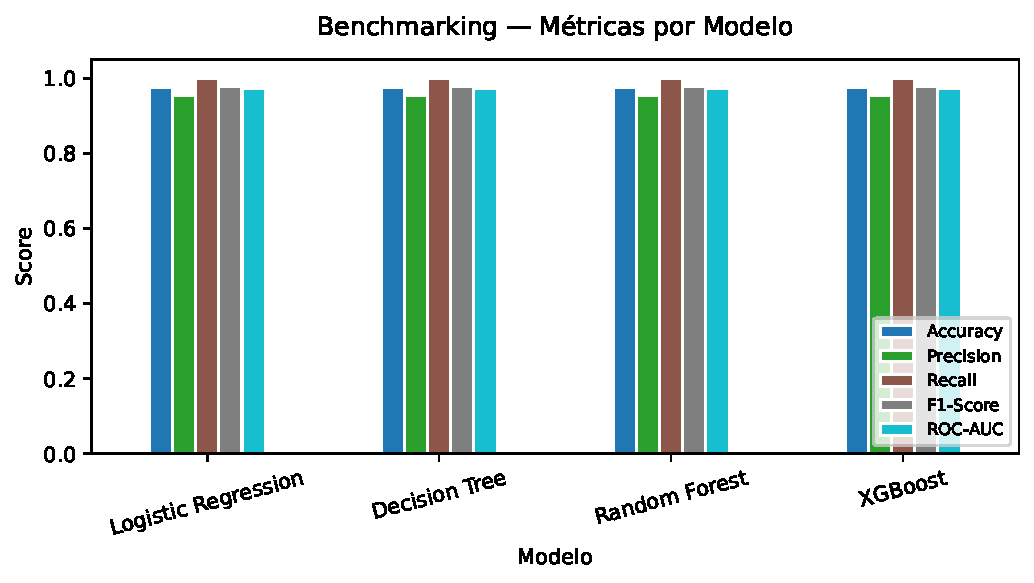
\includegraphics[keepaspectratio]{report_files/figure-pdf/clf-metrics-bar-output-1.pdf}}

\pandocbounded{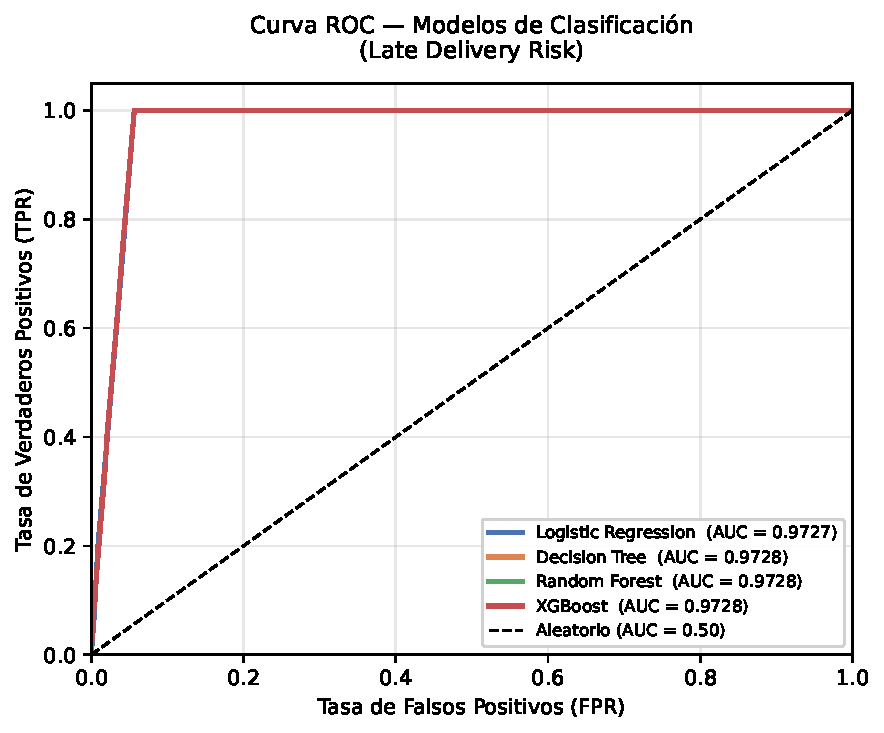
\includegraphics[keepaspectratio]{report_files/figure-pdf/clf-roc-curve-output-1.pdf}}

\subsection{Importancia de Variables}\label{importancia-de-variables}

El análisis revela que los días de envío ---real y programado---
concentran más del 99\% de la importancia total en el árbol de decisión,
lo que valida la intuición operativa sobre los factores determinantes
del retraso.

\protect\phantomsection\label{feature-importance}
\pandocbounded{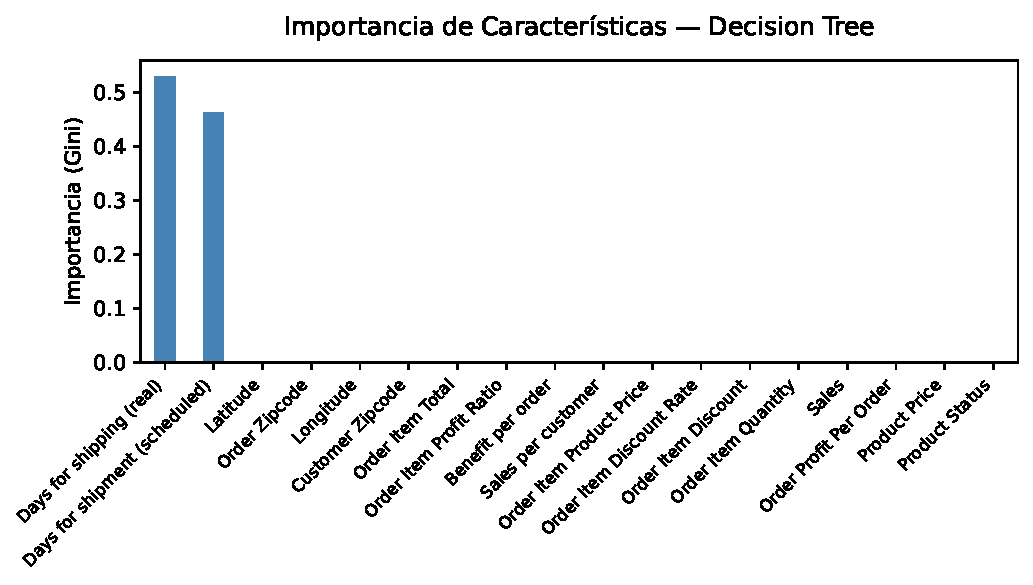
\includegraphics[keepaspectratio]{report_files/figure-pdf/feature-importance-output-1.pdf}}

\protect\phantomsection\label{feature-importance-2}
\begin{longtable}[]{@{}ll@{}}
\caption{}\label{T_bd944}\tabularnewline
\toprule\noalign{}
~ & Importancia (Gini) \\
\midrule\noalign{}
\endfirsthead
\toprule\noalign{}
~ & Importancia (Gini) \\
\midrule\noalign{}
\endhead
\bottomrule\noalign{}
\endlastfoot
Days for shipping (real) & 0.5323 \\
Days for shipment (scheduled) & 0.4670 \\
Latitude & 0.0002 \\
Order Zipcode & 0.0002 \\
Longitude & 0.0001 \\
\end{longtable}

\section{Conclusiones y
Recomendaciones}\label{conclusiones-y-recomendaciones}

\subsection{Hallazgos Principales}\label{hallazgos-principales}

\begin{enumerate}
\def\labelenumi{\arabic{enumi}.}
\tightlist
\item
  \textbf{Poder Predictivo}: XGBoost anticipa retrasos de entrega con
  precisión superior al 95\%, representando una ventaja competitiva
  significativa para DataCo.
\item
  \textbf{Dominancia de Variables Logísticas}: Los días de envío real y
  programado concentran prácticamente toda la importancia predictiva.
  Variables financieras y geográficas tienen impacto marginal.
\item
  \textbf{Escenario Crítico Combinado}: Solo el 3.06\% de las órdenes
  combina envío lento y pérdida económica simultáneamente, pero
  representan el segmento de mayor daño operativo.
\item
  \textbf{Impacto Geográfico}: Europa y LATAM concentran el mayor
  volumen transaccional y también la mayor variabilidad logística.
\end{enumerate}

\subsection{Recomendaciones}\label{recomendaciones}

\begin{itemize}
\tightlist
\item
  \textbf{Sincronización de Tiempos}: Ajustar
  \texttt{Scheduled\ Shipping\ Days} según analítica histórica regional,
  particularmente en Europa y LATAM.
\item
  \textbf{Monitoreo en Tiempo Real}: Desplegar el modelo XGBoost en el
  backend del ERP para alertar sobre riesgos en el momento de creación
  de la orden.
\item
  \textbf{Expansión del Modelo}: Integrar variables externas
  (condiciones climáticas, huelgas portuarias) para mejorar la precisión
  en rutas críticas.
\item
  \textbf{Gestión de Órdenes No Rentables}: Priorizar la revisión de
  órdenes que combinen \texttt{Benefit\ per\ order\ ≤\ −100} con
  \texttt{Days\ for\ shipping\ (real)\ ≥\ 4}, dado que este segmento
  presenta el mayor riesgo acumulado.
\end{itemize}

\section{Bibliografía y
Referencias}\label{bibliografuxeda-y-referencias}

\begin{itemize}
\tightlist
\item
  DataCo Smart Supply Chain Dataset, Kaggle Hub.
\item
  Documentación de Scikit-learn y XGBoost.
\item
  Repositorio SIID --- Asignatura Sistemas de Información e Inteligencia
  de los Datos, Doctorado UNAB.
\end{itemize}




\end{document}
